\chapter{Related work}

In this chapter first pathways are described in general followed by a detailed consideration of pathway visualization and current tools and frameworks. Next the term gene expression is introduced and again state-of-the art framework are described roughly. [Missing introductory sentence for information visualization]. The combination of these two ermerging research areas leads to gene-expression application on biochemical pathways. Finally related work in the field of information visualization that is needed in respect of the former described fields is discussed.

\section{Metabolic Pathway Visualization}

\subsection{Medical Pathways}

[Metabolism is defined in the book Metabolism at a glance and is cited in \citep{Bourqui2006}]

Metabolic networks are defined in \citep{Bourqui2006} as interconnected metabolic pathways.
[Write some more sentences about metabolic networks and why they are important to be investigated globally.]
Figure \stdref{gfx:RocheAppliedScience_MetabolicPathways_WallChart} shows a whole snapshot of a metabolic pathway. The fact that these posters of the global metabolic network are still mounted on the wall in numerous laboratories illustrates why alternative ways of visualization needs to be explored. 

\begin{figure}[ht]
\centering
\scalebox{0.43}{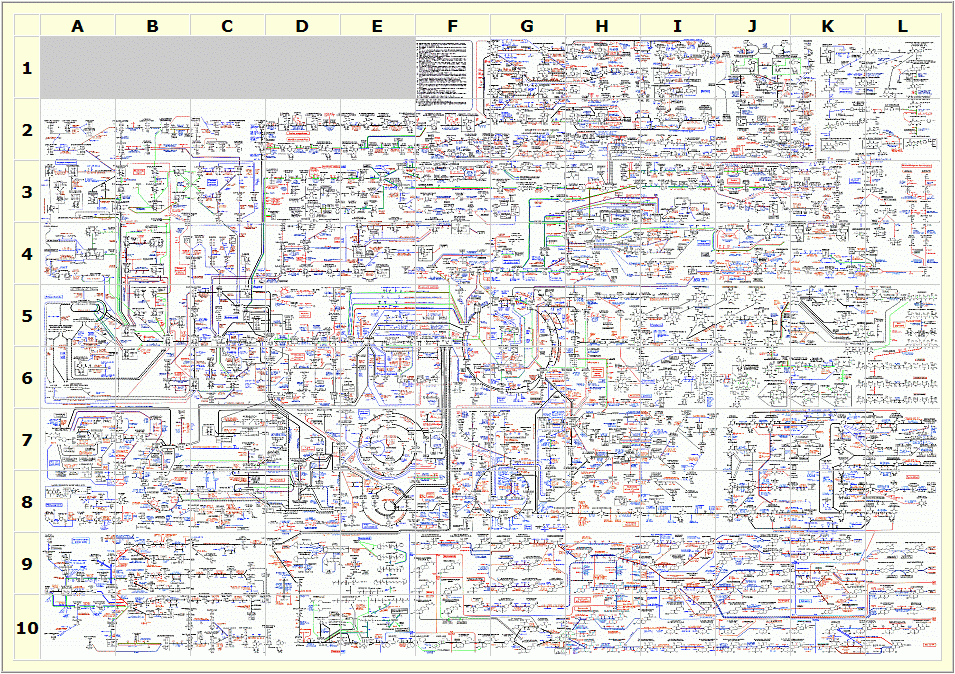
\includegraphics{gfx/RocheAppliedScience_MetabolicPathways_WallChart}} 
\caption[Roche Applied Science wall chart on metabolic pathways]{\textit{Roche Applied Science wall chart on metabolic pathways TODO Insert Reference}} 
\label{gfx:RocheAppliedScience_MetabolicPathways_WallChart}
\end{figure}

\subsubsection{Definition}

Metabolic pathways aim on modelling cellular functions in graphs. Basic building blocks of pathways are chemical compounds (so called metabolites) and enzymes. The chemical compounds act as substrates and products of chemical reactions. Enzymes catalyze these reactions by using substrates as input. The output of the chemical reaction is a product which is in turn a compound. This process is described in LINK. 

Pathways can be divided in metabolic pathways and regulatory pathways such as signal transduction cycles. The former are in the scope of that paper because metabolism can be modeled in reference pathways which are valid for several organisms\citep{Kanehisa2000}. Outgoing from that reference map KEGG can generate organism specific pathways. On the other hand regulatory pathways vary in detail for specific organism and it is much harder to find a common reference pathway\citep{Kanehisa2000}.

[Describe additional information as co-factors etc.]

\subsubsection{Layouting and graph drawing algorithms}

[Defintion of metabolic networks regarding graph theory is presented in \citep{Bourqui2006}.]
A very good explaination of metabolic networks and pathways in respect of graph theory is given by Bourqui et al.\citep{Bourqui2006}.
The metabolic network is a bipartite graph where the set of nodes is divided in two disjoint subsets of nodes whereas no nodes inside a group are connected. In the case of metabolism that means that enzymes are not directly connected to other enzymes. The same applies for chemical compounds. 
Metabolic pathways are partially cyclic graphs. Directed and undirected edges are present.
Nodes can occure in multiple times in the same graph as well as in foreign graphs.

Determined by historical development metabolic networks are often handmade. I.e. experts incorporate their meta-knowledge in the specific domain to position nodes and route edges. Still this approach is widely spread in the community due to the complexity of the graphs. Graph drawing algorithms are needed for automatic generation of pathways. Common graph drawing algorithms do not provide sufficient results in respect of metabolic pathways because they focus on different constraints\citep{Becker2001}. Becker et al. state that common graph layouting alogrithms are optimized to fullfil the following cirterias:
\begin{itemize}
 \item Planarity
 \item Minimal edge crossings
 \item Minimal drawing area
 \item Maximal symmetry
\end{itemize}
In matters of metabolic graphs it is hard to define a simple set of criterias and constraints because the complexity and diversity. Therfore special algorithms need to be developed that are capable of handling the biochemical properties.

One of the first attempts to dynamically model metabolic networks was done by Karp et al. starting in 1993\citep{Karp1993, Karp1994, Karp1994a}. As metabolic network became more and more diversified and complex over time also graph drawing approaches needed to be adapted and enhanced. Becker et al. proposed an algorithm that builds up on the ideas of Kerp et al. and enhances them by including the topological structure. As a starting point the method seeks for the longest cycle inside the graph. The rest of the nodes are classified as inner and outer components which are positioned using a spring embedded algorithm.

In the recently published work by \citep{Bourqui2006} a graph drawing algorithm is published that addresses the visual identification of reaction cascades among distinct metabolic pathways by forming a single concatenated graph [should I put a figure here?].

\subsubsection{2.5D and 3D pathway visualization}


\subsubsection{Pathways visualization using Virtual Reality (VR)}

[Insert short definition of virtual reality - Judith bringt Referenz.]

In 2002 Rojdestvenski et al. (\citep{Rojdestvenski2002, Rojdestvenski2003}) proposed a tool called Metabolic Network Visualizer (MNV) for the usage of virtual reality in context of metabolic pathways by using Virtual Reality Modeling Language (VRML). They also discuss advantages and possible problems when using a real 3D representation of the biomedical network. Finally a hierarchical postitioning of the graphs in 3D space as flat 2D graphs is proposed to keep the 2D graphs with that the biologists are familiar with. 
\citep{Dickerson2003}:[paper contains a good definition of metabolic pathways as graphs]
In \citep{Yang2006} the MetNetVR is presented which focuses on hierarchical relationships in pathways (-> also in \citep{Dogrusoz2004}). The root node of the graph could
be the metabolic network. Childs of the network are several pathways which subnodes are their molecules. For exploring the information space detail-on-demand techique (-> link to other section) is applied. Using a tracked input device orientation and position for  ray-picking in an virtual environment the user can expand a single node pathway representation to show all contained molecules.

\subsection{State-of-the-art Frameworks}

Brandes et al. propesed a 2.5D method to visualize differences accross pathways for different spzecies\citep{Brandes2004}. This method enables the user to see evolutionary developments and relations amoung different species.

\section{Gene Expression Visualization}

\subsection{Gene-Expression Analysis}

Describe the Genome.
Human genome is sequenced since year by name -> Reference 
Describe how genes code enzymes (special proteins).

Hierarchical clustering\citep{Seo2002}

\subsection{State-of-the-art frameworks}

http://www.genome.jp/kegg/expression/

\minisec{GeneSpring}

\begin{figure}[ht]
\centering
\scalebox{0.4}{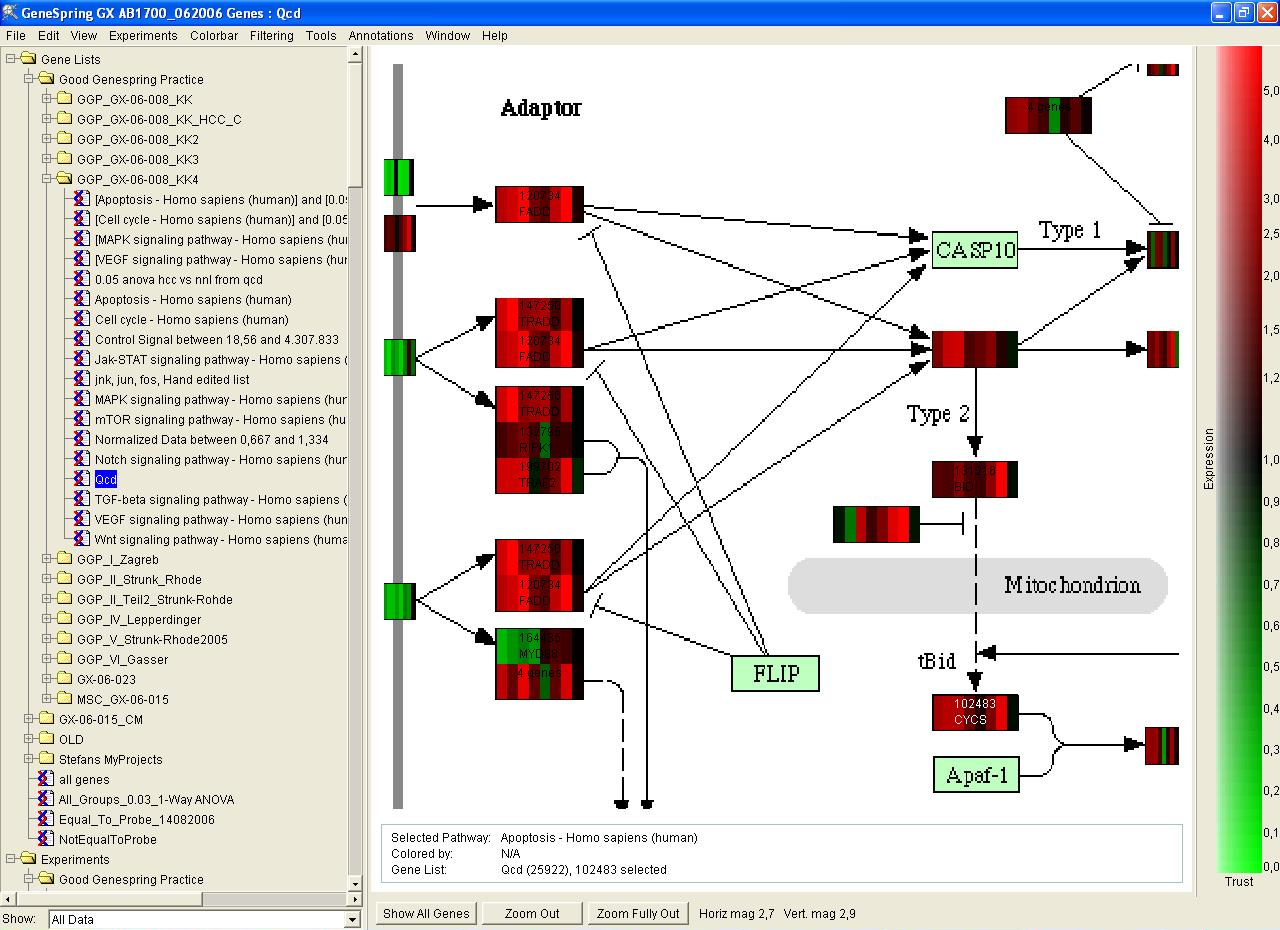
\includegraphics{gfx/screenshot_gene_spring}} 
\caption[Screenshot of GeneSpring]{\textit{Screenshot of GeneSpring}} 
\label{gfx:screenshot_gene_spring}
\end{figure}

\minisec{Panther}

The PANTHER (Protein ANalysis THrough Evolutionary Relationships) classifies genes by functions\footnote{http://www.pantherdb.org}.
[Reference?]

Pathway drawing tool called CellDesigner\footnote{http://www.celldesigner.org}.

\begin{figure}[ht]
\centering
\scalebox{0.4}{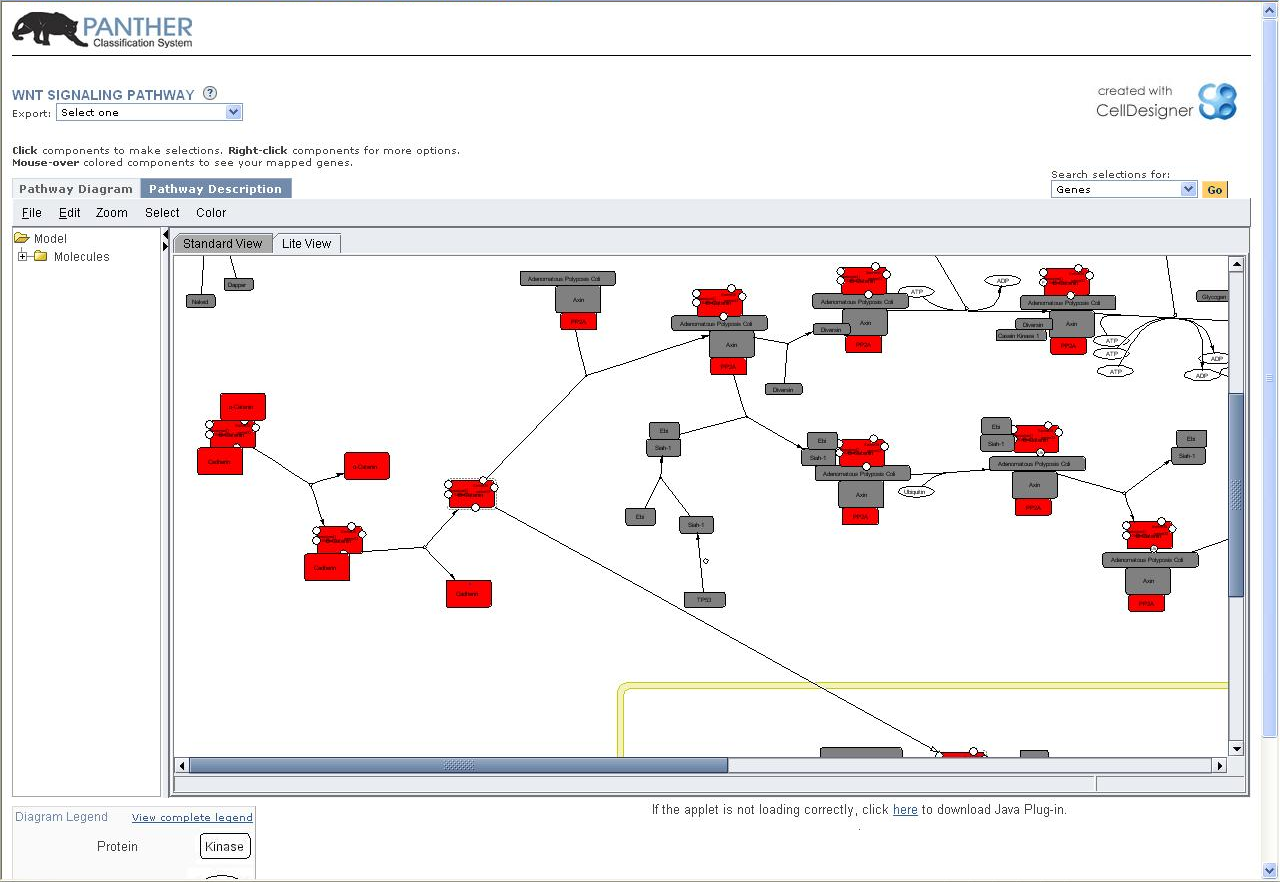
\includegraphics{gfx/screenshot_cell_designer}} 
\caption[Screenshot of CellDesigner]{\textit{Screenshot of CellDesigner}} 
\label{gfx:screenshot_cell_designer}
\end{figure}

\section{Biomedical Databases}

Criterias for successful databases are: 
\begin{itemize}
 \item Availability
 \item Update rate / update process
 \item ID Management (Unique Key)
 \item Links to other databases
 \item Software to access database (SOAP)
 \item Documentation
 \item Full data dump 
 \item etc.
\end{itemize}

\subsection{Gene centered databases}

\subsubsection{International Nucleotide Sequence Database Collaboration (INSDC)}

The INSDC is a collaborative network of DNA sequence databases that consists of three major members:
\begin{itemize}
 \item \textbf{GenBank:} \\
 GenBank is a part of the National Center for Biotechnology Information (NCBI) which is intergrated in the United States National Library of Medicine (NLM). NLM belongs to the National Institutes of Health (NIH) that is self-described as the focal point for medical research in the United States.
 \item \textbf{European Molecular Biology Laboratory (EMBL):} \\
 EMBL
 \item \textbf{DNA Data Bank of Japan (DDBJ)} \\
\end{itemize}

INSERT table with current data sets in various databases
Number of genes, proteins, enzymes.

\subsubsection{Entrez}

\subsubsection{Gene Ontology (GO)}

\subsection{Pathway centered databases}

\subsubsection{Kyoto Encyclopedia of Genes and Genomes (KEGG)}

The Kyoto Encyclopedia of Genes and Genomes (KEGG)\footnote{http://www.genome.jp/kegg/} is a biomedical resource that started its online service in 1995 and belongs to the Japanese GenomeNet.

Provide 140 metabolic pathways for over ?? organisms.

KEGG pathways are represented by graphs which are layouted by hand and stored in static images (reference?). [Images are generated, how?]
ok
In the graph enzymes are visualized by rectangular nodes and compounds are modelled by small circles. Round rectangular nodes depict linked pathways. This circumstance points to the fact that a pathway is only an artificial subset of a huge complex network. 

When a cellular function is valid throughout different organisms it is called strongly preserved. These general pathways are stored in the KEGG database as reference pathways. Each reference pathway can then be specialized for a specific organism. Figure BLA shows the methionine metabolism for home sapiens. Light green color coded enzymes depict proteins where the generating genes are known. 

[Describe possiblities of KEGG in terms of database information and relation browsing - pathway coloring - hierarchical division of metabolic network]

Throughout the paper Methionine Metabolism serves as prime example. This special amino acid pathway is of average size and includes all types of nodes and edges as well as cyclic reaction cascades. \stdref{gfx:KEGG_methionine_metabolism_271_reference_pathway} shows the reference pathways of Methionine Metabolism while \stdref{gfx:KEGG_methionine_metabolism_271_pathway_hsa} depicts the specialized cellular function cycle for homo sapiens. The graphs share the same composition and connection of nodes but vary in the color coding of enzymes. Human genes that produce enzymes in the pathway are highlighted yellowish. 

\begin{figure}[ht]
\centering
\scalebox{0.4}{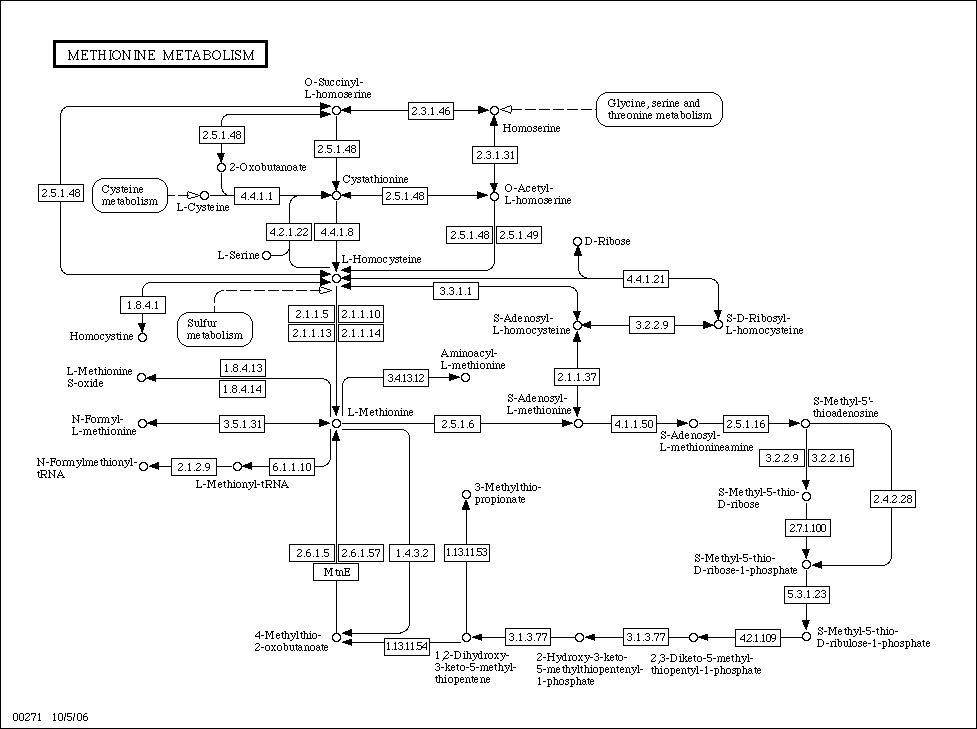
\includegraphics{gfx/KEGG_methionine_metabolism_271_reference_pathway}} 
\caption[KEGG methionine metabolism reference pathway]{\textit{KEGG methionine metabolism reference pathway}} 
\label{gfx:KEGG_methionine_metabolism_271_reference_pathway}
\end{figure}

\begin{figure}[ht]
\centering
\scalebox{0.4}{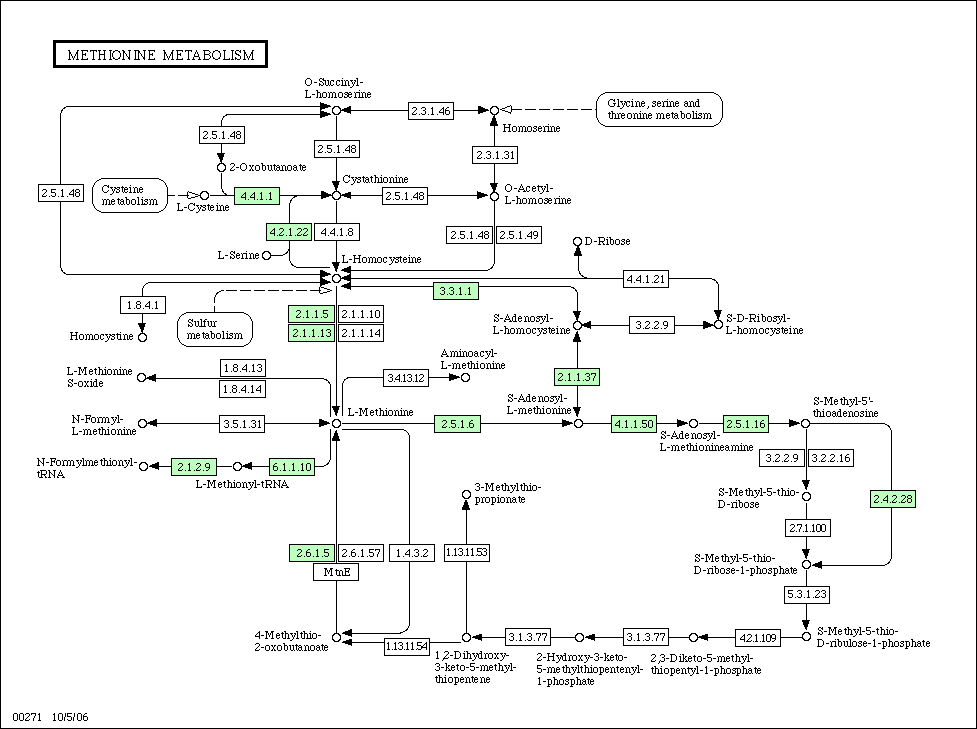
\includegraphics{gfx/KEGG_methionine_metabolism_271_pathway_hsa}} 
\caption[KEGG methionine metabolism pathway for home sapiens]{\textit{KEGG methionine metabolism pathway for home sapiens}} 
\label{gfx:KEGG_methionine_metabolism_271_pathway_hsa}
\end{figure}

\subsubsection{BioCyc}
\subsubsection{ExPASy Molecular Biology Server}

Reference: A new generation of information retrieval tools for biologists: the example of the ExPASy WWW server (Appel et al.)

\subsection{Biomedical Identification Numbers}

During the last decade biochemical database projects sprang up like mushrooms. Some projects has proven their value and achieved to manifest themeselves inside the community. Each database project introduced their own identification numbers for genes, proteins, nucleotids, etc. The obvious problem is how to map these data and interconnect them among the misscellaneous databases. 
There were many attempts over the time to get this issue under control.

\minisec{Enzyme ID}
The Nomenclature Committee of the International Union of Biochemistry and Molecular Biology (NC-IUBMB) agreed on the Enzyme Commission number (EC number)\footnote{http://www.chem.qmul.ac.uk/iubmb/enzyme/}\citep{Bairoch2000}. Enzymes are divided by classes and a couple of subclasses which are seperated by a ``.'' (e.g.: 3.1.1.1). The Enzyme nomenclature database\footnote{http://www.expasy.org/enzyme/} is online provided by the Swiss-Prot platform.
The release of 03-Apr-2007 contains 4026 active entries. 
Each entry contains:
\begin{itemize}
 \item EC-number
 \item Official name
 \item Alternative names
 \item Reactions catalyzed
 \item Co-factors (if any)
 \item Cross-links to other databases
\end{itemize}

\minisec{Gene ID}
The nomenclature for enzymes become widely accepted however inn the case of genes unique identifiers are much more silvered.
Several identifcation systems are still under usage but the main problem is the uniquity of the gene identifiers.

\minisec{Pathway ID}

\section{Information Visualization Methods}

\citep{Bederson2003}
\citep{Spence2007}
\citep{Schumann2000}

\subsection{2D vs. 3D}

\subsection{Multiple Views}

\subsection{Focus + Context}

\subsection{Linking \& Brushing}

\subsection{Detail on demand}

\subsection{Semantic Zooom}

\section{Application of Gene-Expression Data onto Metabolic Pathways}

\subsection{State-of-the-art frameworks}

\minisec{PathwayExplorer [2005]}

The PathwayExplorer is able to map genes on enzymes in pathways from various databases.
Positive: Can handle all kind of identifiers (for example RefSeq, ...).
Negative: Needs time to map genes on pathways. The result are static PNG images.

\begin{figure}[ht]
\centering
\scalebox{0.43}{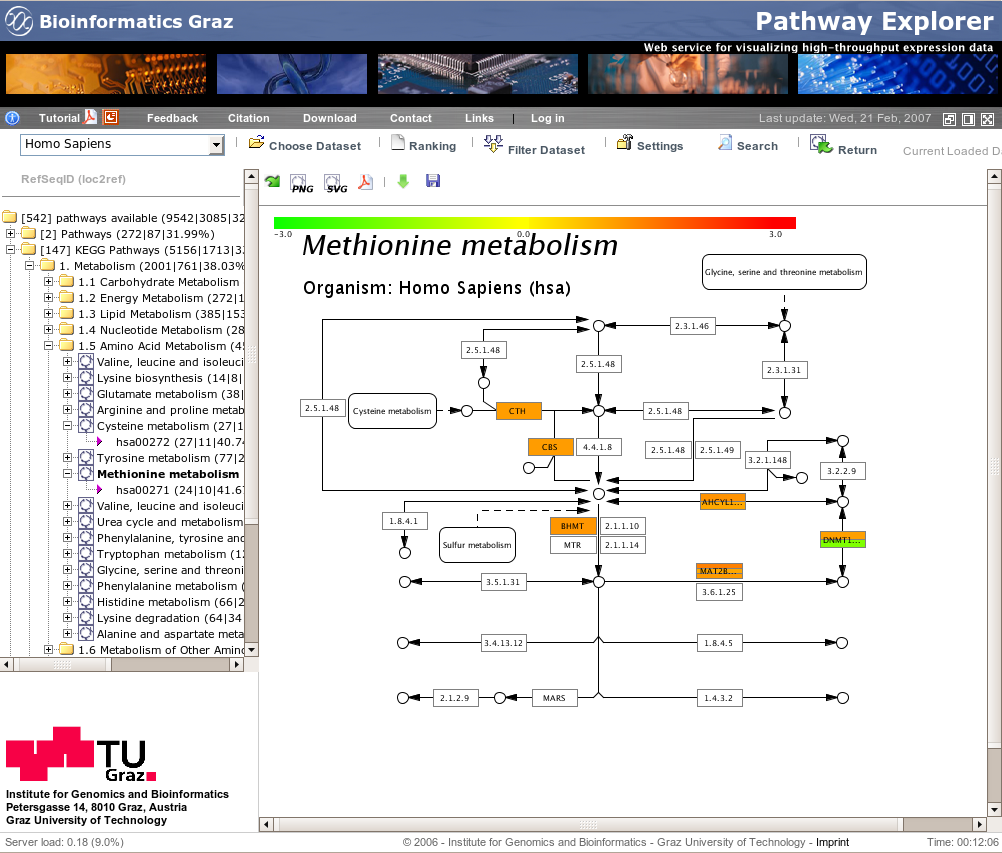
\includegraphics{gfx/screenshot_pathway_explorer}} 
\caption[PathwayExplorer]{\textit{PathwayExplorer}} 
\label{gfx:pathway_explorer}
\end{figure}
